\let\cleardoublepage\clearpage

\chapter{\textit{Blackboard}}\label{sec:blackboard}
\let\cleardoublepage\clearpage

O padrão arquitetural \textit{Blackboard} (ou Quadro-Negro) tem sido amplamente utilizado para enfrentar problemas com características de incerteza \cite{dong2005event}. Muitas vezes, não há solução algorítmica direta para problemas dessa natureza e a melhor solução trata-se de uma aproximação. 

Esta arquitetura se baseia em um repositório central, onde agentes leem e escrevem em um quadro-negro, e um agente mestre controla o que é lido e escrito por estes agentes.
As aplicações deste padrão podem ser encontradas em diferentes tipos de sistemas, como sistemas de comunicação, mobilidade e coordenação.  



\begin{description}
  \item[Nome do padrão:] \textit{Blackboard} ou Quadro-Negro.
    \item[Referências:]    \citeonline{dong2005event}, \citeonline{weiss1999multiagent}, \citeonline{ito2000blackboard}.
    \item[Categoria:] \textit{Simple Structure}.
    \item[Problema:] é adotado em problemas com características de incerteza \cite{dong2005event}, onde não há solução algorítmica direta para o problema e a melhor solução trata-se de uma aproximação. É adotado também para possibilitar o acesso paralelo a dados e a execução simultânea de tarefas.
    \item[Solução:] \citeonline{weiss1999multiagent} apresenta a metáfora a seguir para demonstrar este padrão.

\begin{citacao}"Imagine um grupo de especialistas humanos ou de agentes sentados ao lado de um grande quadro-negro. Os especialistas estão trabalhando cooperativamente para resolver o problema, usando o quadro-negro como local de trabalho para desenvolver a solução. A resolução de problemas começa quando o problema e a data inicial estão escritos no quadro-negro. Os especialistas observam o quadro-negro, procurando uma oportunidade para aplicar seus conhecimentos à solução em desenvolvimento. Quando um especialista encontra informações suficientes para fazer uma contribuição, ele registra a contribuição no quadro-negro. Esta informação adicional pode permitir que outros especialistas apliquem seus conhecimentos. Este processo de adicionar contribuições para o quadro-negro continua até o problema ter sido resolvido."\cite{weiss1999multiagent}
\end{citacao}


Esta metáfora captura uma série de características importantes deste padrão, cada uma das quais são descritas a seguir.

\begin{itemize}
    \item \textbf{Independência da experiência}: os especialistas (chamados de fontes de conhecimento, \textit{Knowledge Sources} ou KSs) não são treinados para trabalhar unicamente com esse grupo específico de especialistas. Cada um é especialista em alguns aspectos do problema e pode contribuir para a solução independentemente da combinação particular de outros especialistas na sala.
    \item \textbf{Diversidade em técnicas de resolução de problemas}: o algoritmo interno de representação e inferência adotado por cada KS é ocultado;
    \item Representação flexível da informação do quadro-negro: não há quaisquer restrições prévias sobre as informações que podem ser colocadas no quadro-negro;
    \item \textbf{Linguagem de interação comum}: os KS devem ser capazes de interpretar corretamente as informações gravadas no quadro-negro por outros KSs. Pode haver tanto uma representação compreensível apenas entre alguns KSs e uma representação genérica compreensível por todos os KSs;
    \item \textbf{Ativação baseada em eventos}: os KSs são acionados em resposta ao quadro-negro e aos eventos externos. Os eventos do quadro negro incluem a adição de novas informações ao mesmo, uma alteração na informação existente ou a remoção de informações existentes. Cada KS informa o sistema de quadro-negro sobre o tipo de eventos em que ele está interessado. O sistema de quadro-negro grava esta informação e considera diretamente o KS a ser ativado sempre que esse tipo de evento vier a ocorrer;
    \item \textbf{Necessidade de controle}: há um componente de controle que é separado dos KSs e é responsável por gerenciar o fluxo  da resolução de problemas. O componente de controle pode ser visto como um especialista na resolução de problemas. Ele analisa o benefício geral das contribuições possíveis pelos KSs para a resolução do problema em questão. Ao ser finalizada a execução de um KS, o componente de controle ativa o KS mais apropriado para execução. Ao ser disparado, o KS utiliza seus conhecimentos para avaliar a qualidade e a importância de sua contribuição. Cada KS disparado informa o componente de controle sobre a qualidade e os custos associados à sua contribuição, sem realmente realizar o trabalho para calcular a contribuição. O componente de controle usa essas estimativas para decidir como proceder, e
    \item \textbf{Geração de solução incremental}: KSs contribuem para a solução conforme apropriado, às vezes refinando, às vezes contradizendo, e às vezes iniciando uma nova linha de raciocínio.
\end{itemize}

%O acoplamento do controle e as políticas de controle não concordam com a separação de preocupações [6], que é um dos principais princípios da engenharia de software. É uma das principais causas de complexidade na arquitetura do quad ro-negro. É difícil mudar o controle de um agente para o outro. As políticas de controle também se tornam difíceis de modificar. Os grandes sistemas multi-agente são necessários para serem confiáveis ​​e sobreviventes. O componente de controle é uma parte crítica dos sistemas. A falha de um agente de controle não deve resultar na falha de todo o sistema. O novo agente deve poder assumir o papel de controle e fazer a transição de forma suave e transparente. Depois que os sistemas foram definidos, a manutenção dos sistemas também é crucial. A evolução e a mudança dos agentes do sistema devem ser suportadas pela arquitetura. A arquitetura dos sistemas multi-agente deve ser capaz de lidar com a evolução para que o impacto sobre as partes do sistema seja isolado e minimizado. Novos agentes são capazes de entrar na fonte ou controle do conhecimento dos sistemas, enquanto os agentes antigos podem deixar os sistemas. Os agentes também são adaptáveis ​​a diferentes \cite{dong2005event}.


Há, portanto, três componentes principais neste padrão \cite{dong2005event}: 

\begin{enumerate}
    \item \textbf{Fontes de conhecimento (ou \textit{Knowledge Sources})}: cada KSs é um especialista na resolução de certos aspectos do problema geral. Uma vez que ele encontra a informação que precisa no quadro-negro, pode prosseguir sem qualquer ajuda de outras fontes de conhecimento; 
    \item \textit{Blackboard} (ou \textbf{Quadro-negro}): o quadro-negro é a fonte de todos os dados em que a fonte de conhecimento irá operar e é o destino para todas as conclusões a partir de uma fonte de conhecimento, e %Existem dois tipos de conhecimento: estático e dinâmico. O conhecimento estático é uma informação imutável de longa duração, enquanto o conhecimento dinâmico é o conhecimento que é gerado durante a execução;
    \item \textbf{Controle}: é um gerente que considera cada solicitação feita à fonte de conhecimento. O controle é responsável por abordar o quadro-negro em termos do que a fonte de conhecimento pode contribuir e o efeito que a contribuição pode ter sobre a solução a ser proposta. O controle tenta manter a resolução de problemas dentro do fluxo correto, de modo a garantir que todos os aspectos cruciais do problema recebam atenção e a equilibrar a importância estabelecida das contribuições dos diferentes especialistas. Os componentes de controle também são fontes de conhecimento, entretanto, se concentram no processo de solução de problemas de domínio específicos. %O controle pode ser implementado invocando diretamente as fontes de conhecimento apropriadas ou invocação de método. Nesse caso, as políticas de controle são codificadas com o controle particular, dificultando a alteração do controle e as políticas de controle de forma independente.
\end{enumerate}

%A função de controle pode ser assumida por diferentes agentes em momentos diferentes. Um agente pode entrar no sistema registrando o controle e deixar o sistema com um novo sucessor para participar. A mudança de controle dinâmica exige que todos os agentes assumam o controle para levar as políticas de controle com eles. Caso contrário, pode haver resultados inesperados ao mudar o controle. Por outro lado, as políticas de controle não são corrigidas e podem ser alteradas ao longo do tempo. Como consequência, cada agente que é possível ser um controle foi notificado para as mudanças. Mais especificamente, existem vários efeitos sobre as propriedades do nível do sistema da arquitetura do software \cite{dong2005event}.


    \item[Modelagem:]  A Figura \ref{fig:blackboard_model} representa a arquitetura básica deste padrão.
    
\begin{figure}[h!]
    \centering
    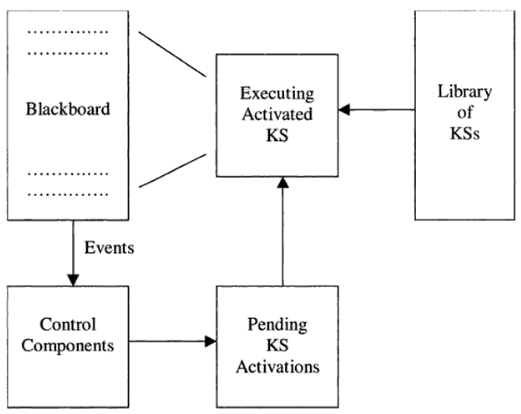
\includegraphics[scale=0.5]{figuras/blackboard/blackboard_model.png}
    \caption{A arquitetura básica de um sistema \textit{Blackboard}. Fonte: \citeonline{weiss1999multiagent}.}
    \label{fig:blackboard_model}
\end{figure}

\begin{comment}
\begin{figure}[h!]
    \centering
    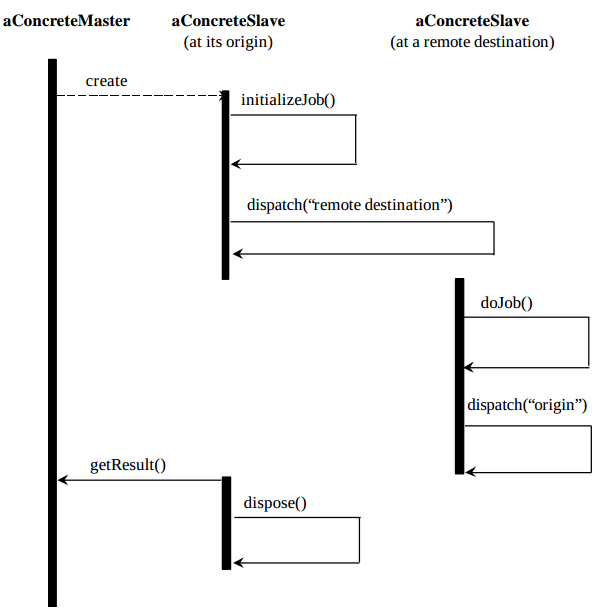
\includegraphics[scale=0.4]{figuras/master_slave/diagrama_sequencia.png}
    \caption{Diagrama de sequência do padrão \textit{Master-Slave}. Fonte: \citeonline{aridor1998agent}}
    \label{fig:master_sl_diagrama_sequencia}
\end{figure}\end{comment}


%Vantagens adicionais do sistema \textit{Blackboard} consistem no acesso paralelo a dados e execução simultânea de tarefas. Introduzir alterações no sistema de quadro-negro como um agente e excluí-lo do sistema torna-se simples. 



%%

\item[Exemplo:] 

De modo a exemplificar uma utilização do padrão \textit{Blackboard}, é apresentado o \textit{Collaborative
Supply Chain System} (CSCS) descrito por \citeonline{ito2000blackboard}. Trata-se de um sistema de gerenciamento de cadeia de suprimentos compreendido em uma rede integrada de membros, são eles: fornecedores, fábricas, armazéns, centros de distribuição e varejistas. Devido à complexidade desta rede, toda a cadeia de processos logísticos necessita ser gerenciada. 

A colaboração entre os membros desempenha um papel crítico para implementar um sistema eficaz, mas sua implementação não seria fácil apenas com o mecanismo convencional de compartilhamento de informações. O intuito é proporcionar uma coordenação mais rápida e mais visível entre uma empresa, seus clientes e fornecedores. O CSCS é projetado para aumentar a velocidade e a certeza da oferta de suprimentos.


Conforme mostrado na Figura \ref{fig:blackboard_example}, cada agente interage e compartilha informações através de um quadro-negro. O quadro-negro regula e fornece informação a cada membro do sistema, são eles: \textit{Supplier Agent} (SA), \textit{Manufacturer Agent} (MA), \textit{Distributor Agent} (DA) e \textit{Customer Agent} (CA). A colaboração destes membros e a introdução de técnicas de negociação são desempenhadas por duas redes:

\begin{itemize}
    \item \textit{Intranet}: pode ser usada de modo a fornecer serviços de comunicação interna para obter melhores resultados do que os meios convencionais de acesso e transferência de dados. Por meio do \textit{Manufacturer Agent}, os usuários acessam informações diárias, e a empresa pode facilmente exibir informações críticas de usuários externos.  Basicamente, o \textit{Manufacturer Agent}  atua no controle de inventário regulando os níveis de inventário e negocia com os outros agentes para facilitar a circulação de materiais. A distribuição destes materiais é designada pelo \textit{Distributor Agent}, e 
    \item \textit{Internet}: é uma base unificada composta por todos os membros do sistema e que permite que os usuários se comuniquem para as trocas de informações. Por exemplo, a \textit{Internet} pode ser usada para oferecer a oportunidade de comparar  fornecedores, escolher um fornecedor adequado e garantir que o fornecedor selecionado satisfaça os requisitos.
\end{itemize}

\begin{figure}[h!]
    \centering
    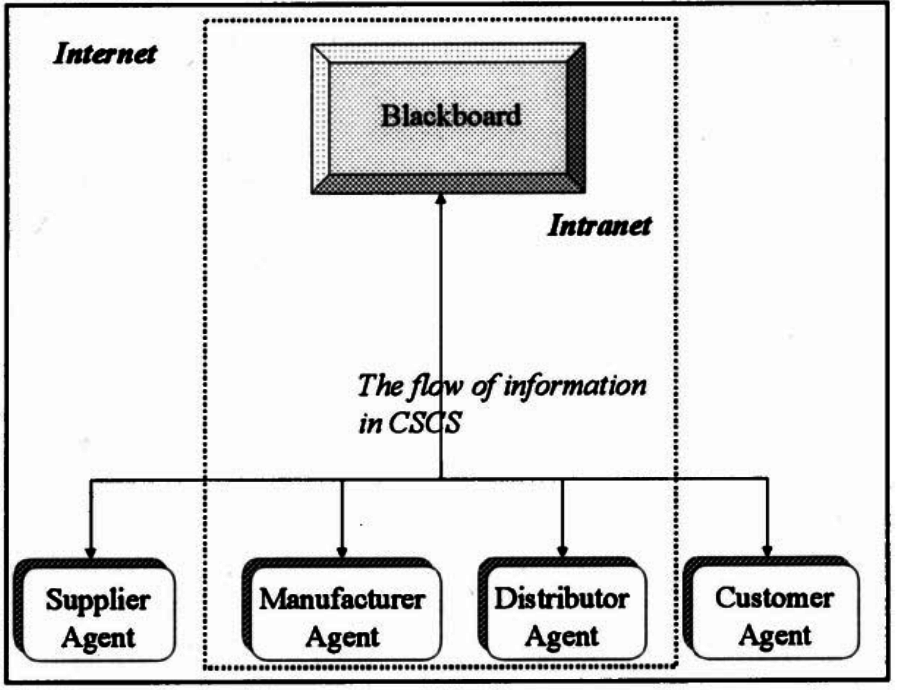
\includegraphics[scale=0.30]{figuras/blackboard/blackboard_example.png}
    \caption{Interação entre agentes no CSCS. Fonte: \citeonline{ito2000blackboard}.}
    \label{fig:blackboard_example}
\end{figure}

As empresas são obrigadas a cumprir as ordens dos clientes mesmo quando é difícil fazê-lo. Elas devem responder às ordens de forma rápida e eficiente dentro do tempo limitado e disponível para atender às solicitações de suprimentos de seus clientes.

Ordens que surgem de modo imprevisto e com urgência, quando ocorrem, causam atraso na entrega e diminuem a eficácia dos membros do sistema. A colaboração dos membros do CSCS e a introdução de técnicas de negociação fornecem uma solução para esses problemas.

Suponha-se que para a reposição de peças e materiais, uma empresa publica um leilão no quadro-negro. Este leilão pode ser visualizado por toda a comunidade de fornecedores, caracterizando-se, portanto, como uma competição aberta. 

Os agentes fornecedores, \textit{Supplier Agents}, de cada empresa fornecedora, exploram a Internet para encontrar os leilões de seu interesse. Quando um agente encontra um leilão de seu interesse, ele indica sua respectiva companhia fornecedora.

Em seguida, o quadro-negro publica os lances apresentados por estas companhias. Os membros realizam revisões dos lances ou negociam com essas empresas. Logo após, o lance mais apropriado é selecionado com base em critérios de seleção. 

Se por ventura um problema de entrega ocorre com um dos fornecedores, os agentes colaboram e negociam entre si para substituí-lo. O fornecedor alternativo é escolhido de acordo com os critérios de seleção preparados pelo fabricante (\textit{Manufacturer Agent}). A Figura \ref{fig:blackboard_process} mostra como esses tipos de atividades ocorrem quando o fornecedor selecionado não entregar os materiais no momento certo. Nessa atividade, o fornecedor em questão, o fabricante e o fornecedor alternativo são controlados pelo \textit{Supplier Agent} 1 (SA1), \textit{Manufacturer Agent} (MA) e \textit{Supplier Agent} 2 (SA2), respectivamente.

\begin{figure}[h!]
    \centering
    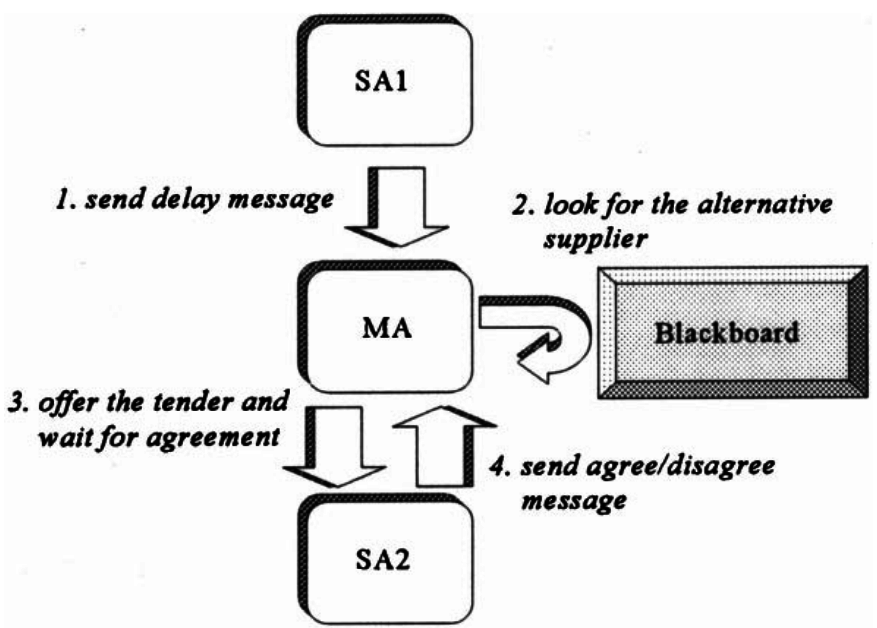
\includegraphics[scale=0.30]{figuras/blackboard/blackboard_process.png}
    \caption{Processo de colaboração e negociação para substituição de fornecedor. Fonte: \citeonline{ito2000blackboard}.}
    \label{fig:blackboard_process}
\end{figure}


Quando o problema acontece, o SA1 envia uma mensagem de atraso para o MA. Depois de receber a mensagem de atraso, o MA refere-se ao BB para fornecer um fornecedor alternativo para a substituição. Se o SA2 for considerado o fornecedor alternativo, o MA faz uma consulta ao SA2 e solicita a estimativa de custo da entrega.

Então, o SA2 cita o custo dos materiais e o tempo da entrega estimado e os envia de volta ao MA. Se o SA2 não aceitar a oferta, o MA executará o mesmo procedimento para outro fornecedor alternativo. E deste modo, são realizadas as atividades de colaboração e negociação entre esses agentes, ajudando fabricantes e fornecedores a resolver os problemas durante o processo de entrega.

\item[Implementação:] a fim de demonstrar o padrão \textit{Blackboard}, é utilizado o contexto acima para simular a entrega de materiais. Todos os detalhes da implementação, configuração de ambiente e passos para execução são descritos no Apêndice \ref{appendix:blackboard}.

\end{description}

